\documentclass[tikz,border=5pt]{standalone}
\usepackage{pgfplots}
\usepackage{amsmath}
\usepackage{siunitx}
\usepackage{xcolor}

\usetikzlibrary{arrows}
\usetikzlibrary{arrows.meta}
\usetikzlibrary{calc}

% original colors
\definecolor{color1}{RGB}{166,118,29}
\definecolor{color2}{RGB}{217,95,2}
\definecolor{color3}{RGB}{231,41,138}
\definecolor{color4}{RGB}{117,112,179}
\definecolor{color5}{RGB}{27,158,119}
\definecolor{color6}{RGB}{102,166,30}
\definecolor{color7}{RGB}{230,171,2}


\begin{document}
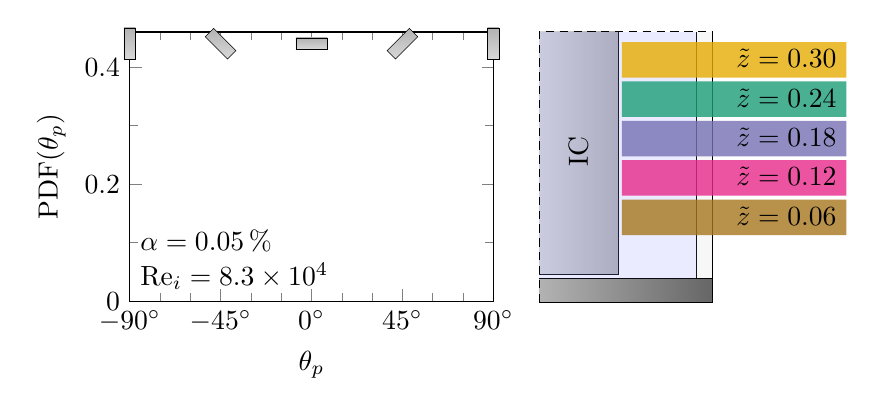
\begin{tikzpicture}
  [
    rec0/.style={shade,
                rectangle,
                minimum width=4mm,
                minimum height=1.5mm,
                inner sep=0pt,
                outer sep=0pt,
                top color=gray!60!white,
                bottom color=gray!30!white,
                draw=black, 
                very thin},
    rec45/.style={shade,
                rectangle,
                rotate=45,
                minimum width=4mm,
                minimum height=1.5mm,
                inner sep=0pt,
                outer sep=0pt,
                top color=gray!60!white,
                bottom color=gray!30!white,
                draw=black, 
                very thin},
    rec45r/.style={shade,
                rectangle,
                rotate=-45,
                minimum width=4mm,
                minimum height=1.5mm,
                inner sep=0pt,
                outer sep=0pt,
                top color=gray!60!white,
                bottom color=gray!30!white,
                draw=black, 
                very thin},
    rec90/.style={shade,
                rectangle,
                rotate=90,
                minimum width=4mm,
                minimum height=1.5mm,
                inner sep=0pt,
                outer sep=0pt,
                top color=gray!60!white,
                bottom color=gray!30!white,
                draw=black, 
                very thin}
  ]
  \begin{axis}[
    name=main,
    clip mode=individual,
    xmin=-90, xmax=90,
    ymin=0,
    ymax=0.46,
    enlargelimits=false,
    axis on top=false,
    xlabel=$\theta_p$,
    ylabel=$\text{PDF}(\theta_p)$,
    %legend pos=south east,
    legend style={draw=none, 
                  font=\scriptsize,
                  fill=none,
    },
    legend style={at={(0, 0)}, anchor=south west},
    legend cell align=left,
    %reverse legend,
    width = 6.2cm,
    height = 5.0cm,
    ylabel near ticks,
    xtick={-90, -45, 0, 45, 90},
    xticklabels={\ang{-90}, \ang{-45}, \ang{0}, \ang{45}, \ang{90}},
    minor ytick={0.1, 0.3},
    minor xtick={-75, -60, -30, -15, 15, 30, 60, 75}
  ]

  %\addplot+[
    %color=color1,
    %mark=none,
    %very thick,
    %line join=round,
   %] table [
    %x = bins,
    %%y = hist,
    %y expr = \thisrow{hist} * (180/3.14159265359),
    %col sep=comma,
%] {orientation_0.06.csv};
%%\addlegendentryexpanded{$0.1 < r \leq 0.3$}

  %\addplot+[
    %color=color3,
    %mark=none,
    %very thick,
    %line join=round,
   %] table [
    %x = bins,
    %%y = hist,
    %y expr = \thisrow{hist} * (180/3.14159265359),
    %col sep=comma,
%] {orientation_0.12.csv};
%%\addlegendentryexpanded{$0.3 < r \leq 0.5$}

  %\addplot+[
    %color=color4,
    %mark=none,
    %very thick,
    %line join=round,
   %] table [
    %x = bins,
    %%y = hist,
    %y expr = \thisrow{hist} * (180/3.14159265359),
    %col sep=comma,
%] {orientation_0.18.csv};
%%\addlegendentryexpanded{$0.5 < r \leq 0.7$}

  %\addplot+[
    %color=color5,
    %mark=none,
    %very thick,
    %line join=round,
   %] table [
    %x = bins,
    %%y = hist,
    %y expr = \thisrow{hist} * (180/3.14159265359),
    %col sep=comma,
%] {orientation_0.24.csv};
%%\addlegendentryexpanded{$0.7 < r \leq 0.9$}

  %\addplot+[
    %color=color7,
    %mark=none,
    %very thick,
    %line join=round,
   %] table [
    %x = bins,
    %%y = hist,
    %y expr = \thisrow{hist} * (180/3.14159265359),
    %col sep=comma,
%] {orientation_0.3.csv};
%\addlegendentryexpanded{$0.7 < r \leq 0.9$}

  % Plot reference particles
  \path (axis cs: 0,   0.44) coordinate[rec0];  
  \path (axis cs: 45,  0.44) coordinate[rec45];  
  \path (axis cs: -45, 0.44) coordinate[rec45r];  
  \path (axis cs: -90, 0.44) coordinate[rec90];  
  \path (axis cs: 90,  0.44) coordinate[rec90];  

 \end{axis}


 \begin{scope}[
     %scale=3,
     %every node/.append style={transform shape},
     xshift=52mm,
     yshift=3.4mm,
    ]
    %\clip (-0.487, -1.220) rectangle (0.502, -1.9);
    \newcommand{\icheight}{30.8mm}
    \newcommand{\icwidth}{10mm}
    \newcommand{\platewidth}{22mm}
    \newcommand{\plateheight}{3mm}
    \newcommand{\icplategap}{0.5mm}
    \newcommand{\octhickness}{2mm}
    \newcommand{\icbeamgap}{0.5mm}
    \newcommand{\beamwidth}{4.5mm}
    \newcommand{\beamextend}{17mm}
    \newcommand{\beamhe}{25mm}
    \newcommand{\beamhd}{20mm}
    \newcommand{\beamhc}{15mm}
    \newcommand{\beamhb}{10mm}
    \newcommand{\beamha}{5mm}
    
    % ic
    \fill[
     color=gray,
     shade,
     inner sep=0pt,
     outer sep=0pt,
     right color=gray!60!white,
     left color=gray!30!white,
    ] (0, 0) -- (0, \icheight) -- (\icwidth, \icheight) -- (\icwidth, 0) --
      (0, 0);
    \draw[very thin, black] (0, 0) -- (\icwidth, 0) -- (\icwidth, \icheight);

    % bottom plate
    \fill[
     color=gray,
     shade,
     inner sep=0pt,
     outer sep=0pt,
     right color=black!60!white,
     left color=black!30!white,
    ] (0, -\icplategap) -- (\platewidth, -\icplategap) --
    (\platewidth, -\icplategap-\plateheight) -- (0, -\icplategap-\plateheight)
    -- (0, -\icplategap);
    \draw[very thin, black] (0, -\icplategap) -- (\platewidth, -\icplategap) --
    (\platewidth, -\icplategap-\plateheight) -- (0, -\icplategap-\plateheight);

    % oc
    \fill[
     color=gray!20,
     opacity=0.3,
     inner sep=0pt,
     outer sep=0pt,
    ] (\platewidth, -\icplategap) -- (\platewidth, \icheight) --
      (\platewidth-\octhickness, \icheight) -- 
      (\platewidth-\octhickness, -\icplategap) --
      (\platewidth, -\icplategap);
    \draw[very thin, black] (0, 0)
        (\platewidth-\octhickness, \icheight) -- 
        (\platewidth-\octhickness, -\icplategap) --
        (\platewidth, -\icplategap) -- (\platewidth, \icheight);

    % water
    \fill[
     color=blue!40,
     opacity=0.2,
     inner sep=0pt,
     outer sep=0pt,
    ] (0, -\icplategap) -- (\platewidth-\octhickness, -\icplategap) --
      (\platewidth-\octhickness, \icheight) -- 
      (0, \icheight) -- (0, -\icplategap);

    % side cut-off lines (dashed lines)
    \draw[black, densely dashed] (0, -\icplategap-\plateheight) --
       (0, \icheight) -- (\platewidth, \icheight);

    % laser beams
    \fill[
     color=color1,
     opacity=0.8,
    ] (\platewidth+\beamextend, \beamha) -- (\icwidth+\icbeamgap, \beamha) --
      (\icwidth+\icbeamgap, \beamha) --
      (\icwidth+\icbeamgap, \beamha+\beamwidth) -- 
      (\platewidth+\beamextend, \beamha+\beamwidth);
    \node[align=right, anchor=south east]
    at (\platewidth+\beamextend,\beamha) {$\tilde{z}=0.06$};

    \fill[
     color=color3,
     opacity=0.8,
     ] (\platewidth+\beamextend, \beamhb) -- (\icwidth+\icbeamgap, \beamhb) --
       (\icwidth+\icbeamgap, \beamhb) --
       (\icwidth+\icbeamgap, \beamhb+\beamwidth) -- 
       (\platewidth+\beamextend, \beamhb+\beamwidth);
    \node[align=right, anchor=south east]
    at (\platewidth+\beamextend, \beamhb) {$\tilde{z}=0.12$};

    \fill[
     color=color4,
     opacity=0.8,
    ] (\platewidth+\beamextend, \beamhc) -- (\icwidth+\icbeamgap, \beamhc) --
      (\icwidth+\icbeamgap, \beamhc) --
      (\icwidth+\icbeamgap, \beamhc+\beamwidth) -- 
      (\platewidth+\beamextend, \beamhc+\beamwidth);
    \node[align=right, anchor=south east]
    at (\platewidth+\beamextend, \beamhc) {$\tilde{z}=0.18$};

    \fill[
     color=color5,
     opacity=0.8,
    ] (\platewidth+\beamextend, \beamhd) -- (\icwidth+\icbeamgap, \beamhd) --
      (\icwidth+\icbeamgap, \beamhd) --
      (\icwidth+\icbeamgap, \beamhd+\beamwidth) -- 
      (\platewidth+\beamextend, \beamhd+\beamwidth);
    \node[align=right, anchor=south east]
    at (\platewidth+\beamextend, \beamhd) {$\tilde{z}=0.24$};

    \fill[
     color=color7,
     opacity=0.8]
      (\platewidth+\beamextend, \beamhe) -- (\icwidth+\icbeamgap, \beamhe) --
      (\icwidth+\icbeamgap, \beamhe) --
      (\icwidth+\icbeamgap, \beamhe+\beamwidth) -- 
      (\platewidth+\beamextend, \beamhe+\beamwidth);
   \node[align=right, anchor=south east]
   at (\platewidth+\beamextend, \beamhe) {$\tilde{z}=0.30$};

   %z=0
   %\draw[thick, red, line cap=round]
    %(\platewidth, -\icplategap) -- (\platewidth+1.5mm, -\icplategap);
   %\node[align=left, anchor=east]
        %at (\platewidth+12.5mm, 0) {$z=0$};
    % camera
    %\begin{scope}[
            %xshift=2.75cm,
            %yshift=-1cm
        %]
        %\fill[
        %color=blue!10,
        %draw=black,
        %line width=0.1mm,
        %rounded corners=1mm] (0,0.17) -- (-0.25, 0.05) -- (-0.25, 0.45) -- (0,
        %0.33);
        %\fill[
        %color=blue!10,
        %draw=black,
        %line width=0.1mm,
        %rounded corners=1mm] (0,0) rectangle (1, 0.5);
    %\end{scope}
    
    \node[anchor=west, rotate=90] at (5mm, 12.5mm) {IC};

 \end{scope}

 \node[anchor=south west] at (0.01, 0.5) {$\alpha=\SI{0.05}{\percent}$};
 \node[anchor=south west] at (0.01, 0.02) {$\text{Re}_i=\num{8.3e4}$};
 
\end{tikzpicture} 
\end{document}
